%Author: Niels Meyering
% University of Osnabrück
%
\RequirePackage{atbegshi}

\documentclass[12pt]{article}

\usepackage[utf8]{inputenc}
\usepackage[german,ngerman]{babel}
\usepackage{grffile}
\usepackage{rotating}
\usepackage{amsthm}
\usepackage{amsmath}
\usepackage{parskip}
\usepackage{fixltx2e}

\usepackage{url}

\usepackage{graphicx}
%\makeatletter\let\l@addto@macro\relax\makeatother
% Textspiegel
\usepackage{typearea}
\areaset[0.75cm]{16cm}{21cm}
\addtolength{\topmargin}{1cm}
\RequirePackage[bf,small,margin=1.0cm]{caption}

%\makeatletter\let\l@addto@macro=\relax\makeatother
%\usepackage[skip=0cm,list=true,labelfont=it]{subcaption}
\usepackage{subcaption}

\newtheorem{definition}{Definition}

\usepackage{hyperref}
%\usepackage{biblatex}
\bibliographystyle{plain}
%\usepackage{tikz}
%\PreviewEnvironment{tikzpicture}
%\setlength\PreviewBorder{5pt}%

\begin{document}

\title{Solar CSP}
\author{Niels Meyering\\ Energiesystemanalyse, SS 2013\\ Institut Umweltsystemforschung, Universität Osnabrück}
\date{August 2013}

\begin{titlepage}

\newcommand{\HRule}{\rule{\linewidth}{0.5mm}} % Defines a new command for the horizontal lines, change thickness here

\center % Center everything on the page
 
%----------------------------------------------------------------------------------------
%	HEADING SECTIONS
%----------------------------------------------------------------------------------------

\textsc{\LARGE Universität Osnabrück}\\[1.5cm] % Name of your university/college
\textsc{\Large Energiesystemanalyse SS 2013}\\[0.5cm] % Major heading such as course name
\textsc{\large }\\[0.5cm] % Minor heading such as course title

%----------------------------------------------------------------------------------------
%	TITLE SECTION
%----------------------------------------------------------------------------------------

\HRule \\[0.4cm]
{ \huge \bfseries Solar CSP }\\[0.4cm] % Title of your document
\HRule \\[1.5cm]
 
%----------------------------------------------------------------------------------------
%	AUTHOR SECTION
%----------------------------------------------------------------------------------------

\begin{minipage}{0.3\textwidth}
\begin{flushleft} \large
\emph{eingereicht von:}\\
Sascha Kolodzey\\
Niels Meyering
\end{flushleft}
\end{minipage}
~
\begin{minipage}{0.6\textwidth}
\begin{flushright} \large
\emph{Dozent:} \\
Dr. Peter Viebahn\\
\end{flushright}
\end{minipage}\\[4cm]

% If you don't want a supervisor, uncomment the two lines below and remove the section above
%\Large \emph{eingereicht von:}\\
%Sascha Kolodzey,\\
%Niels Meyering\\[3cm] % Your name

%----------------------------------------------------------------------------------------
%	DATE SECTION
%----------------------------------------------------------------------------------------

{\large August 2013}\\[3cm] % Date, change the \today to a set date if you want to be precise

%----------------------------------------------------------------------------------------
%	LOGO SECTION
%----------------------------------------------------------------------------------------

%\includegraphics{Logo}\\[1cm] % Include a department/university logo - this will require the graphicx package

\includegraphics[height=2cm]{unilogo.png}
 
%----------------------------------------------------------------------------------------

\vfill % Fill the rest of the page with whitespace

\end{titlepage}

\tableofcontents
\newpage

\section{Einleitung}
Solarthermie (Concentrated Solar Power (CSP)) ist eine vielversprechende erneuerbare Energiequelle f�r die Zukunft. Das Verfahren zur Energiegewinnung nutzt die Sonnenstrahlung zur Gewinnung von W�rme, um diese dann durch Gas oder Dampfmaschinen in elektrische Energie umzuwandeln. In den letzten Jahren hat die Technik zunehmend an Aufmerksamkeit gewonnen, was Gro�projekten wie Desertec und Euromed best�tigen. Zum jetzigen Zeitpunkt existieren unterschiedliche Technologien zur Nutzung der Sonnenstrahlung. F�r die Zukunft stellen sich also die Fragen, f�r welche Regionen sich eine Technologie auf lange Sicht am besten eignet, welche Kapazit�ten installiert werden m�ssen und wie viel Energie �berhaupt erzeugt werden kann. Desweitern m�ssen ebenfalls Techniken zur Speicherung der Energie bei geringer Nachfrage entwickelt und getestet werden. All diese Punkte stehen nat�rlich in direktem Zusammenhang mit �konomischen und �kologischen Kosten, die es zu analysieren gilt. Die derzeitigen Prognosen zur Marktentwicklung von sehen bis 2015 einen Anteil von etwa 12 GW durch Sorarthermie gewonnen Strom vor.

\section{Technologien und Technische Entwicklung}
CSP Anlagen beziehen ihre prim�re Energiequelle aus der Direct Normal Irradiance (DNI), welche im besten Fall in einem rechten Winkel zu einer Oberfläche ausgerichtet ist, die in der Lage ist die Sonnenstrahlung aufzunehmen. Dieses Potential ist im sogenannten "`sun belt"' am größten. Der "`sun belt"' bezeichnet den Bereich der Erde nördlich und südlich vom zwanzigsten bis zum vierzigsten Breitengrad. Zum jetzigen Zeitpunkt wurden vier Haupttechnologien entwickelt und getestet:

\begin{itemize}
	\item Parabolrinnenkraftwerke
	\item Fresnelrinnenkraftwerke
	\item Solarturmkraftwerke
\end{itemize}

\begin{figure}[H]
	\centering
	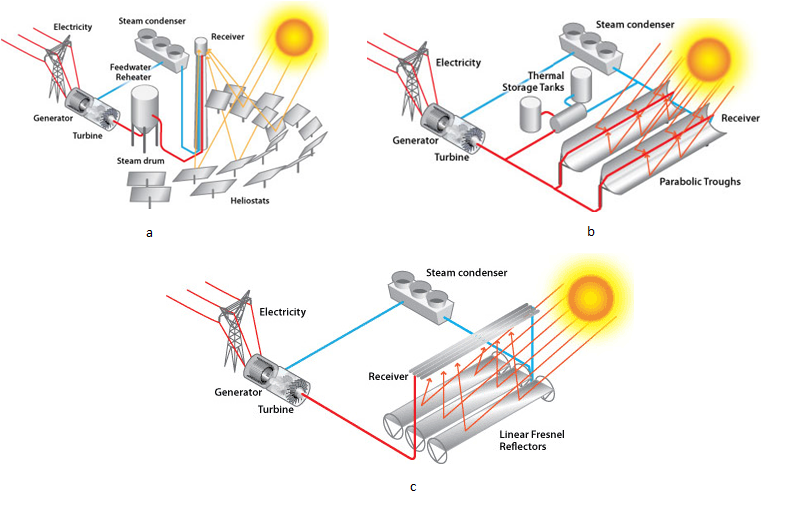
\includegraphics[width=0.9\textwidth]{technik.png}
	\caption{CSP Technologien}
	\label{fig:technik}
\end{figure}

\textbf{Parabolrinnenkraftwerke}
\newline
Ein Parabolrinnenkraftwerk besteht aus einer Reihe von parabelförmigen Sonnenkollektoren und einer Gasturbine zur Erzeugung von elektrischer Energie. Zur Überführung der Wärmeenergie von den Kollektoren zur Turbine wird eine Transferflüssigkeit verwendet. Diese besteht meistens aus einem synthetisch hergestellten Öl, welches durch die Kollektoren fließt. Das Öl wird im Anschluss zur Erzeugung von heißem Dampf genutzt, was schlussendlich durch die Turbine strömt. Für die Zukunft werden neue Technologien im Bereich der Transferflüssigkeit angestrebt. So sind Lösungen ohne den Gebrauch von Öl erstrebenswert, da die Verwendung von Öl mit hohen Kosten in der Aufbereitung und Entsorgung verbunden ist. Auch ist die Verwendung von geschmolzenem Sand in der Entwicklung, welches gegenüber Öl eine höhere Effizienz erzielt, da weitaus höhere Temperaturen erreicht werden können.

\textbf{Fresnelrinnenkraftwerke} 
\newline
Im Gegensatz zu Parabolrinnenkraftwerke setzen Fresnelrinnenkraftwerke auf ebene Kollektoren, die im Gegensatz zur Parabolkollektoren die Sonnenstrahlung auf nur einer Achse aufnehmen. Dies hat eine Effizienzminderung zu Folge, da nicht alle Bereiche des Kollektors orthogonal zur Strahlenrichtung ausgerichtet sind. Die Idee der Fresnel Technologie besteht darin, dass durch die Vereinfachte Technik und die dadurch geringeren Kosten den Verlust der Energie kompensieren.

\textbf{Solarturmkraftwerke}
\newline
Solarturmkraftwerke bestehen aus einem Feld von  Kollektoren, die leicht geneigt die Sonnenstrahlung auf einen in der Mitte des Feldes befindlichen Turm reflektieren. Im Turm werden die gebündelten Strahlen dazu genutzt um wieder eine Transferflüssigkeit zu erhitzen, welche zur Erzeugung von Dampf genutzt wird. Ein Vorteil bei diesem Ansatz gegenüber oben Genannten, ist der geringe Transportweg der Energie bis zu Erzeugung von elektrischer Energie. Die Turbine befindet sich meistens direkt im Turm selbst, sodass keine langen Transportwege nötig sind.
\newline

\begin{figure}[H]
	\centering
	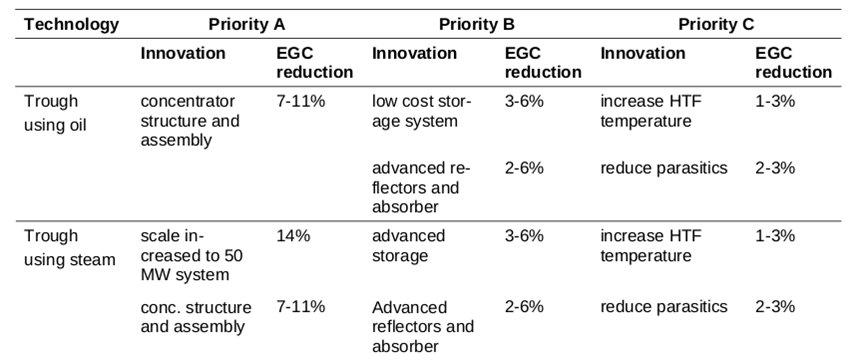
\includegraphics[width=0.9\textwidth]{technische_entwicklung1.png}
	\caption{Technische Entwicklung 1}
	\label{fig:technik_e1}
\end{figure}

Allgemein sind technische Entwicklungen für die Zukunft vor allem in den Bereichen Reflektoren, Speicher, Skalierbarkeit und Temperatur anzusehen \ref{fig:technik_e1}.

\newline
Reflektoren k�nnen in Bezug auf Widerstandsf�higkeit, Reflektionsgrad, Wirkungsgrad, Gewicht und Zusammenbau weiter optimiert werden. Desweitern besteht Innovationspotential für neue Transferflüssigkeiten, die zum Transport der W�rme n�tig sind.

\begin{figure}[H]
	\centering
	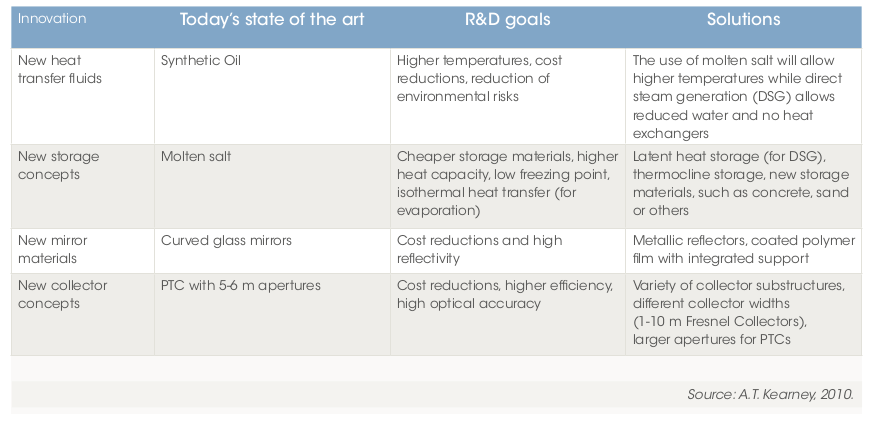
\includegraphics[width=0.9\textwidth]{technische_entwicklung2.png}
	\caption{Technische Entwicklung 2}
	\label{fig:technik_e2}
\end{figure}

\newline
Um die gewonnene Energie zwischen zu speichern sind moderne Speichertechniken gefragt. Hier gibt es ebenfalls neue Konzepte, die mit geschmolzenem Sand arbeiten um eine h�here Hitze Kapazit�t als herk�mliche Speichermedien zu gew�hrleisten \ref{fig:technik_e2}




\subsection{Technisches und wirtschaftliches Potenzial}
Die zukünftige Entwicklung von CSP lässt sich in zwei Phasen kategorisieren. Zuerst muss eine kommerzieller Anreiz und eine Wettbewerbsfähigkeit auf dem Energiemarkt geschaffen werden. Sollte dies geschehen sein, werden in der zweiten Phase Investoren bereit sein in neue Anlagen zu investieren, was zu einer erhöhten Kapazität führt und somit eine Senkung der Kosten mit sich trägt. Die zweite Phase ist unter normalen Umständen eine Folge einer erfolgreichen Etablierung der Technologie aus Phase Eins. Somit liegt der Schlüssel für eine positive Entwicklung in Phase eins. Um einen kommerziellen Anreiz und Wettbewerb für CSP zu erlangen ist eine aktive Förderung der Technologien bis zu einem kritischen Punkt nötig. Um diesen Punkt zu erreichen sind vor allem die Bereiche von Wichtigkeit, die die ökonomischen Eigenschaften eines CSP Projektes betrachten.
Für eine Entwicklung für die Zukunft wurden von der NEEDS (New Energy Externalities Developments for Sustainability) drei verschiedene Szenarien unter Berücksichtigung von verschiedenen Konditionen aufgestellt. Es wird hierbei zwischen einer "`optimistic-realisitc"' Variante und zwei extremen Varianten "`very optimistic"' und "`pessimistic"' unterschieden. Die Szenarien orientieren sich an dem oben vorgestellten Zwei-Phasen Ansatz.

\begin{figure}[H]
	\centering
	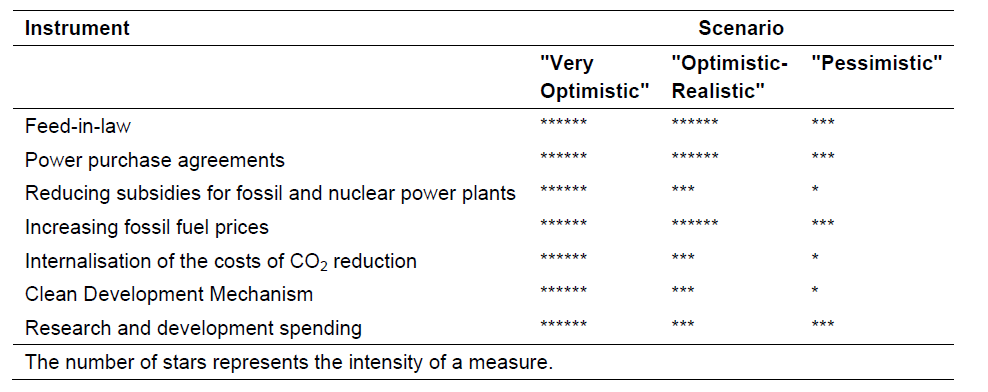
\includegraphics[width=0.9\textwidth]{instruments_scenario.png}
	\caption{Instrumente}
	\label{fig:inst}
\end{figure}

Für die Szenarien wird eine Liste von Parametern aufgestellt, die für jedes Szenario unterschiedliche Gewichte erhalten \ref{fig:inst}.

Das "`very optimistic"' Szenario nimmt an, dass in beide Phasen das volle Potential erreicht wird. In der ersten Phase wird also ein früher Anstieg von CSP Kapazitäten erwartet. Hierzu ist ein globale Klimaschutz Abkommen notwendig, welches alle erneuerbaren Energien enthält und ein Regelwerk vorsieht.
Zum Vergleich sieht das "`optimistic-realistic"' Szenario sieht kein unmittelbares Erreichen aller möglichen Potentiale in Phase eins vor. Es geht davon aus, dass sich diese jedoch im Laufe der Zeit aktivieren. Desweiteren wird nicht davon ausgegangen, dass nukleare und fossile Energien völlig verdrängt werden. Durch Einspeisegesetze, unterstützt durch erhöhten Preise für nukleare und fossile Energien, wird jedoch Anstieg von CSP prognostiziert.
Der Ansatz für das "`pessimistic"' Szenario sieht eine Verzögerung der Entwicklung von CSP um weitere Dekaden vor. In Phase eins wird der kritische Punkt nicht erreicht und es wird zu keiner fördernden Entwicklungsphase, noch zu einer resultierenden Phase zwei kommen. CSP Anlagen werden nicht völlig aus den erneuerbaren Energien verschwinden, jedoch wird nur ein geringer Anstieg bis 2050 vorhergesehen.


\begin{figure}[H]
	\centering
	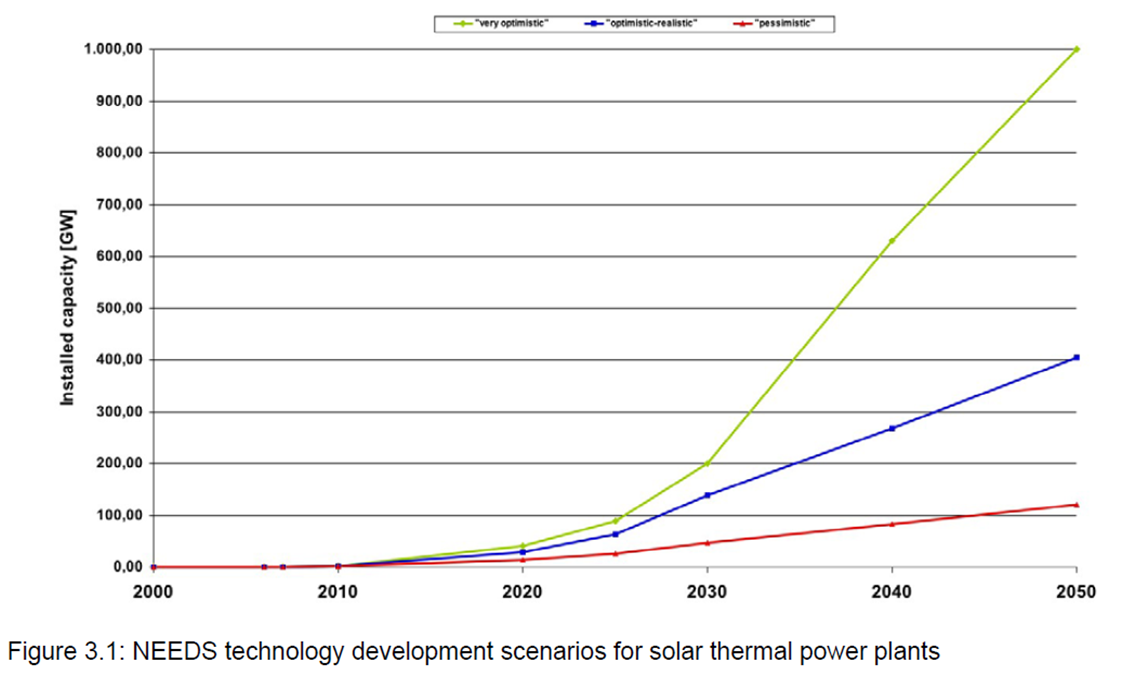
\includegraphics[width=0.9\textwidth]{szenarien.png}
	\caption{Szenarien}
	\label{fig:scenes}
\end{figure}




\section{Kostenanalyse}
\begin{figure}
	\centering
	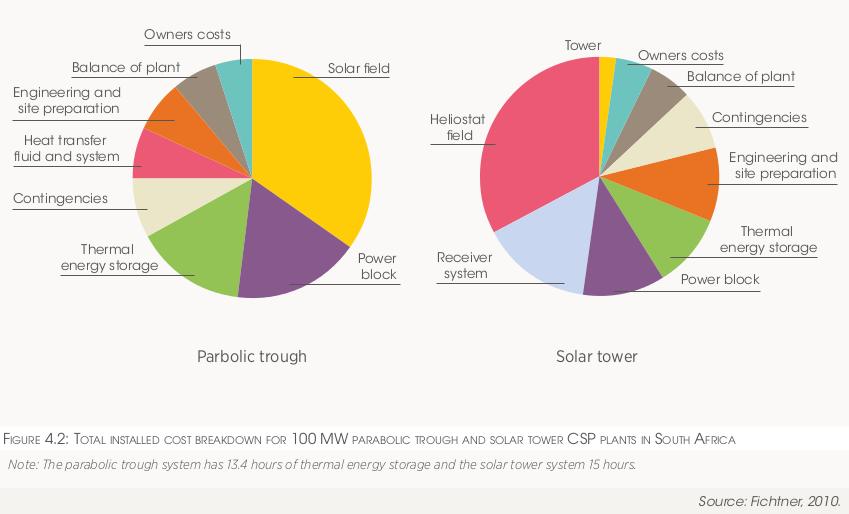
\includegraphics[width=0.9\textwidth]{kostenverteilung.png}
	\caption{Kostenverteilung CSP-Kraftwerke}
	\label{fig:kostenverteilung}
\end{figure}

Der größte Anteil der Kosten eines CSP-Kraftwerks liegt in der initialen Investition bei etwa 80\,\% der Gesamtkosten~\cite{irena2012}. Der Rest der Kosten verteilt sich auf Betrieb und Wartung sowie Versicherung des Kraftwerks.

Die IRENA schätzt die Investitionskosten auf derzeit 4500 - 7150 USD/kWh für ein Solarthermiekraftwerk ohne Wärmespeicher und auf 5000 - 10500 USD/kWh für solche mit Wärmespeicher.

Eine genauere Aufschlüsselung der Investitionskosten zeigt Abbildung~\ref{fig:kostenverteilung}. Der größte Anteil bei Parabolrinnenkraftwerken fällt dabei auf das "`Solar Field"', also den Reflektor-Teil des Kraftwerks. Bei Kraftwerken mit mehr thermischem Speicher sinkt dieser relative Anteil, weil die Speicherkomponente ebenfalls einen erheblichen Teil ausmacht.

\subsection{Zukünftige Entwicklung}

\begin{figure}
	\centering
	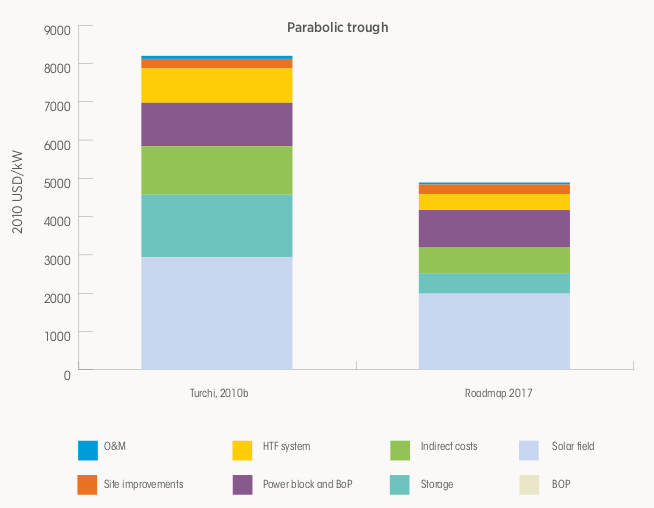
\includegraphics[width=0.9\textwidth]{kostenentwicklung1.png}
	\caption{Voraussichtliche Kostenentwicklung laut IEA CSP-Roadmap 2010}
	\label{fig:kostenentwicklung1}
\end{figure}

\begin{figure}
	\centering
	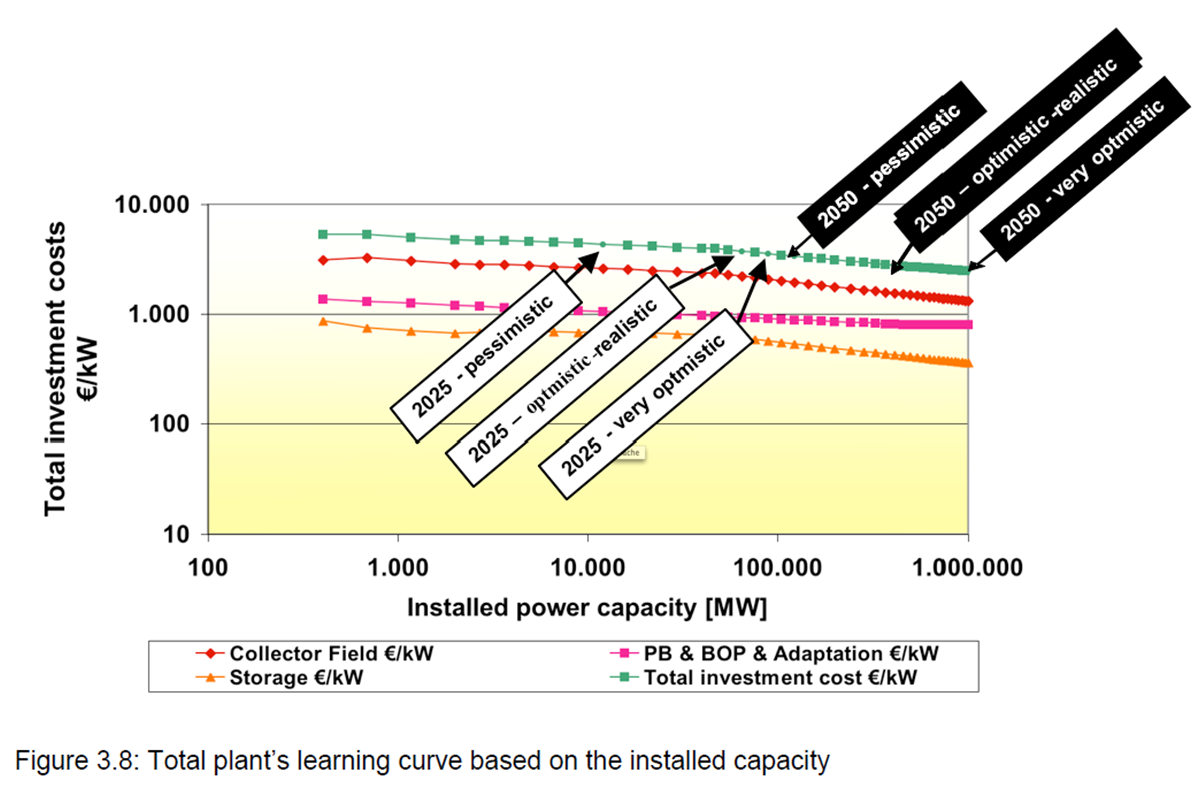
\includegraphics[width=0.9\textwidth]{kostenentwicklung2.png}
	\caption{Kostenentwicklung/Lernkurven basierend auf der installierten Kapazität}
	\label{fig:kostenentwicklung2}
\end{figure}

Die Technology Roadmap der IEA~\cite{iea2010} erwartet eine Reduktion der Kosten bis 2020 zwischen 17\,\% und 40\,\%. Abbildung~\ref{fig:kostenentwicklung1} zeigt die Kostenentwicklung eines Parabolrinnenkraftwerks bis 2017 basierend auf den Ergebnissen eines Kostenmodells auf Grundlage eines 100MW-Referenzkraftwerks in Queensland.
Für Solarturmkraftwerke wird eine Reduktion der Gesamtkosten um etwa 28\,\% bis 2020 erwartet.

Zusätzlich zu diesen Kostenprognosen basierend auf Modellrechnungen gibt es Schätzungen für die allgemeine Lernrate für CSP, also die Reduktion der Kosten je Verdopplung der installierten Kapazität. In Abbildung~\ref{fig:kostenentwicklung2} sind verschiedene Lernkurven dargestellt, basierend auf unterschiedlichen Referenzszenarien~\cite{viebahn2008}. Lernraten von 8-10\,\% werden als konservativ-realistisch angesehen.

Vorsichtige Schätzungen der Stromentstehungskosten (\emph{Levelised Cost of Electricity}, LCOE) liegen derzeit bei 0,20 bis 0,33\,USD/kWh für Parabolrinnen- und zwischen $0,16$ und $0,27$\,USD/kWh für Solarturmkraftwerke. Dies ist im Vergleich mit anderen Techniken ein hoher Wert. Bis 2020 wird je nach Szenario mit einer Reduktion der Stromentstehungskosten auf wettbewerbsfähigere Werte zwischen 0,08 bis 0,16\,USD/kWh gerechnet.\cite{irena2012}



\section{Ökobilanzen}

\section{Ökobilanzen}
Test.

%\subsection{Akzeptanz}

%akzeptanz, wirtschaltiche bedeutung für deutschland
\section{Fazit}

\nocite{viebahn2011}
\nocite{iea2010}
\nocite{irena2012}
\nocite{trieb2009}
\nocite{stegen2012}
\nocite{estela2010}
\nocite{muhlenhoff2010}

\newpage
\bibliography{quellen}

\end{document}
